\documentclass[12pt,a4paper]{article} 
\usepackage[utf8]{inputenx} 
\usepackage[spanish]{babel} 
\usepackage[left=2cm,right=2cm,top=2cm,bottom=2cm]{geometry}
\usepackage{scrextend}
\usepackage{marvosym}
\usepackage{pifont} % Generación de símbolos especiales
\usepackage{textcomp}
\usepackage{newpxtext}
\usepackage{newpxmath}
\usepackage[T1]{fontenc} % Codificación de salida    
\usepackage{microtype} % Mejoras de microtipografía en la obtención de PDF (sólo para pdflatex)
\usepackage[hyphens]{url} % Para escritura de URL
\urlstyle{sf} % Estilo de URL sin serifas para que tengan un mejor aspecto
\usepackage{tikz}
% Paquetes para obtener un mayor control de las listas
\usepackage{paralist} % Mayor control de listas
\usepackage{multicol} % Elementos en varias columnas
\usepackage[breaklinks]{hyperref}
\usepackage{graphicx}
\usepackage{caption}

\usepackage{listings}
\usepackage{color}

\definecolor{dkgreen}{rgb}{0,0.6,0}
\definecolor{gray}{rgb}{0.5,0.5,0.5}
\definecolor{mauve}{rgb}{0.58,0,0.82}

\lstset{frame=tb,
  language=Java,
  aboveskip=3mm,
  belowskip=3mm,
  showstringspaces=false,
  columns=flexible,
  basicstyle={\small\ttfamily},
  numbers=none,
  numberstyle=\tiny\color{gray},
  keywordstyle=\color{blue},
  commentstyle=\color{dkgreen},
  stringstyle=\color{mauve},
  breaklines=true,
  breakatwhitespace=true,
  tabsize=3
}

\captionsetup[figure]{labelformat=empty}
\author{ Iván Illán Barraya \and Javier Monescillo Buitrón}
\title{Construcción de un analizador léxico y sintáctico para un sublenguaje de Java}
\date{\today}
%%%%%%%%%%%%%%

\begin{document}
	
	\maketitle
	
	\begin{figure}[h]
		\centering
		
\includegraphics[width=0.25
		\linewidth]{img/uclm}
		\caption{}
		\label{fig:image004}
	\end{figure}

	\newpage
	\tableofcontents
	\newpage
	
\section{Introducción}
Java \cite{JGosling} es un lenguaje de programación de propósito general, concurrente y orientado a objetos que fue diseñado específicamente para tener las mínimas dependencias de implementación. Su intención principal es permitir que los desarrolladores de aplicaciones escriban el programa una única vez y lo ejecuten el cualquier dispositivo.
\newline\newline
Lo que quiere decir que el código ejecutado en una plataforma no tiene que ser recompilado para correr en otra, así que se puede decir que es un lenguaje compilado e interpretado.
Además Java es uno de los lenguajes de programación más populares en uso, particularmente para aplicaciones de cliente-servidor en la web.
\newline\newline
Esto último hace que sea el lenguaje perfecto para poder introducirlo en el problema que se quiere resolver.


\section{Descripción del problema}
El problema que se presenta es la construcción de un analizador léxico y sintáctico del lenguaje Java usando las herramientas Jflex y Cup \cite{rojas2005java}.\newline\newline
El lenguaje que se propone es un sublenguaje de Java, en concreto una secuencia de métodos en Java que denotaremos como Jjava.

\section{Solución propuesta}
Para diseñar dichos analizadores, utilizaremos los conocimientos de la materia durante las distintas etapas del proceso.

\begin{itemize}
	\item Diseño del sistema
	\item Diseño del Analizador Léxico  \begin{itemize}
		\item Identificar Tokens
		\item Construcción del Analizador Léxico
	\end{itemize}
	
	\item Diseño del Analizador Sintáctico  \begin{itemize}
		\item Especificación de la GLC
		\item Construcción de la gramática con Cup
	\end{itemize}
	
\end{itemize}
La primera etapa consta del diseño referente al lenguaje fuente o arquitectura general del sistema, incluido hasta el análisis léxico. Se proporcionará un diagrama total del problema.
Mientras que para la segunda etapa se trata el análisis sintáctico.
\clearpage
\section{Diseño del sistema}
Para la estructura general del problema se proporciona una pequeña figura \cite{draw} donde se puede ver intuitivamente el funcionamiento del mismo.

\begin{figure}[h]
	\centering
	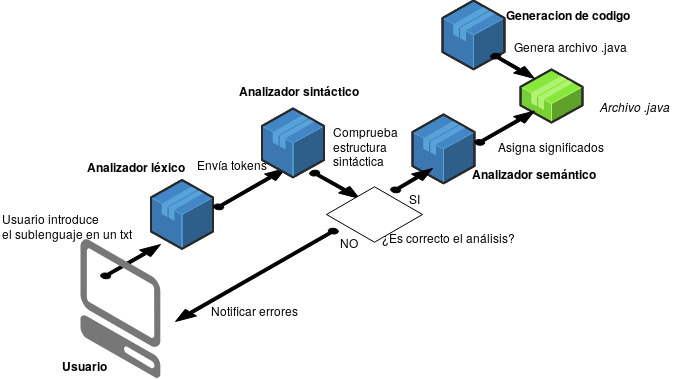
\includegraphics[width=0.9\linewidth]{img/Diagrama_sistema}
	\caption{Diagrama general}
	\label{fig:diagrama-sistema}
\end{figure}

Actualmente la parte de análisis semántico y generación de código no consta dentro del problema pero se incluye para futuras ampliaciones. Se limitará al mismo a la creación de la fase de análisis léxico y análisis sintáctico.

\subsection{Lenguaje fuente}
En esta tabla se pretende dar una descripción inicial de los elementos que tendrá el lenguaje. 
\begin{center}
\begin{tabular}{|c|c|}
	\hline 
	\textbf{Elementos del lenguaje} & \textbf{Ejemplo} \\ 
	\hline 
	Tipos de datos & int o boolean  \\
	\hline 
 	Instrucción de asignación & type\_var a = b; | type\_var a = 0; | c = b; \\
	\hline 
	Decremento & var--; \\ 
	\hline 
	Incremento & var++; \\
	\hline 
	Bucles  &  for( int i = 0; i<hola.length; i++){   /* Ops*/}  \\
	\hline
	Llamadas a métodos & hola = calcularCosas(); | metodoVoid(); \\

	\hline 
 	Retorno de valores &  return x;  \\ 
	\hline  
	Secuencia de instrucciones & a = b; \\
	&  b * 2; //etc \\
	\hline
	Operaciones aritméticas  &  a + b; a - b; a * b; a / b;  \\
	\hline
	Operaciones relacionales & a < b; a <= b; a >= b; a > b; a == b; a!=b;\\
	\hline
	Operaciones lógicas & a \&\& b  a || b y !a \\
	\hline
	Cabecera de los métodos & public static \\
	\hline
	Tipo devuelto de un método & int, boolean, void \\
	\hline
	
\end{tabular} 
\end{center}

Notese, que para cerrar una sentencia es necesario de indicar al final de dicha sentencia el carácter ';' como se hace típicamente en Java.


\subsection{Tabla de tokens}
En la siguiente tabla de tokens, se muestran los lexemas de ejemplo, los tokens y las expresiones regulares asociadas a cada token.
\begin{center}
		\begin{tabular}{|c|c|c|}
			\hline 
			\textbf{Token} & \textbf{Lexema} & \textbf{Patrón} \\ 
			\hline 
			return & return & r$\cdot$e$\cdot$t$\cdot$u$\cdot$r$\cdot$ n  \\ 
			\hline 
			for & for & f$\cdot$o$\cdot$r \\ 
			\hline 
			int & int & i$\cdot$n$\cdot$t \\ 
			\hline 
			boolean	& boolean & b$\cdot$o$\cdot$o$\cdot$l$\cdot$e$\cdot$a$\cdot$n \\ 
			\hline 
			void	& void & v$\cdot$o$\cdot$i$\cdot$d \\ 
			\hline 
			public static	& public static & p$\cdot$u$\cdot$b$\cdot$l$\cdot$i$\cdot$c$\cdot$ $\cdot$s$\cdot$t$\cdot$a$\cdot$t$\cdot$i$\cdot$c \\ 
			\hline 
			true	& true & t$\cdot$r$\cdot$u$\cdot$e \\ 
			\hline 
				false	& false & f$\cdot$a$\cdot$l$\cdot$s$\cdot$e \\ 
			\hline 
			Asignación	& = & = \\ 
			\hline
			Negación	& ! & ! \\ 
			\hline
			Lógicos binarios	& \&\& &  \&$\cdot$\& | |$\cdot$| \\ 
			\hline
			Incrementos	& ++ &  +$\cdot$+ | -$\cdot$- \\ 
			\hline
			Relacionales	& < &  < | <$\cdot$= | > | >$\cdot$= | =$\cdot$= | !$\cdot$= \\ 
			\hline
			Paréntesis abierto	& ( & ( \\ 
			\hline 
			Paréntesis cerrado	& ) & ) \\ 
			\hline 
			Llave abierta	& $\{$ & $\{$ \\ 
			\hline 
			Llave cerrada	& $\}$ & $\}$ \\ 
			\hline 
			Punto y coma	& ; & ; \\ 
			\hline 
			Coma	& , &  , \\ 
			\hline
			Punto	& . &  . \\ 
			\hline
			Asterisco barra & $\ast/$  & $\ast$$\cdot/$ \\ 
			\hline 
			Barra asterisco & $/\ast$  &  $/$$\cdot$$\ast$ \\ 
			\hline  
			ID	& hola  & [A-Za-z][A-Zaz0-9$\_$]* \\ 
			\hline 
				NUM	& 4  & 0 | [1-9][0-9]* \\ 
			\hline
				Valor nulo	& null  & n$\cdot$u$\cdot$l$\cdot$l \\ 
			\hline  
			
		
		\end{tabular} 	
	\end{center}

%Descomentar una vez hecho el EBNF para la entrega 2 :)
%\subsection{EBNF}
HABLAR DE LA NOTACION EXTENDED BACKUS NAUR FORM poner la gramática nueva
Por último, en la siguiente figura puede ver una representación de la gramática del lenguaje en EBNF.

			\begin{center}
			\begin{tabular}{lcl}
	

				PROGRAMA & ::= & DEC$\_$COMP AUTOMATA $\{$AUTOMATA$\}$ \\ 
				 
				
				DEC$\_$COMP & ::= &CMP  CODIGO $\{$ CMP CODIGO $\}$ \\ 
			
				CODIGO 	&::= &'$\#$' ASCII '$\#$' \\ 
				
				AUTOMATA & ::= & \textbf{moore} ID CUERPO$\_$AUTOMATA \\
				
			
				CUERPO$\_$AUTOMATA	& ::= & $'\{'$ ESTADOS ESTADO$\_$INI ALF$\_$IN  \\ 
				
					& &  ALF$\_$OUT TRANSICION COMPORTAMIENTOS $'\}'$ \\ 
				
				ESTADOS	& ::= &   \textbf{estados} $\{$ ID ',' $\}$ ID ';'\\ 
				
				 ESTADO$\_$INI &::= & \textbf{estado$\_$in} ID ';'\\ 
				 
				ALF$\_$IN &::= & \textbf{alf$\_$in}  $\{$ EVENTOS ',' $\}$ EVENTOS ';' \\ 
				
				ALF$\_$OUT & ::= &\textbf{alf$\_$out}  $\{$ CMP ',' $\}$ CMP ';'  \\ 
				
				TRANSICION 	 & ::= & \textbf{transicion} $'\{'$ TRANSICION$\_$DEF $\{$ ',' TRANSICION$\_$DEF  $\}$ ';' $'\}'$ \\ 
				
				TRANSICION$\_$DEF & ::= & '(' ID ',' ID ',' ID ')' \\ 
			
				
				COMPORTAMIENTOS	 & ::= &  \textbf{comportamientos} $'\{'$ COMP$\_$DEF $\{$ ',' COMP$\_$DEF $\}$ ';' $'\}'$\\ 
				
				COMP$\_$DEF &  ::= & '(' ID ',' ID ',' ID ')' \\ 
				
				
				CMP  & ::= & 'c'NUMEROS \\ 
				
				NUMEROS &::= & 0 | 1 | .. | 9 \\ 
				
				COMENTARIOS & ::=  & $'/\ast'$ ASCII $'\ast/'$ \\
				
				
			\end{tabular} 	
		\end{center}
	
	\clearpage


\section{Análisis léxico}
El analizador léxico tiene varias funciones:
\begin{itemize}
	\item Reconocer los símbolos que componen el texto fuente.
	\item Eliminar comentarios del texto fuente.
	\item Eliminar espacios en blanco, saltos de línea, tabulaciones, etc.
	\item Informar de los errores léxicos detectados
\end{itemize}

Como salida del analizador léxico, se obtiene una representación de la cadena de entrada en forma de cadena de \textbf{tokens}, que será posteriormente utilizada en la fase de análisis sintáctico. Para construir el analizador léxico se ha utilizado JFlex. 
\newline
\newline
\textit{JFlex} \cite{flex} es una herramienta software en la que se declaran los tokens que componen nuestro lenguaje fuente, así como las expresiones regulares asociadas a los mismos para poder generar el analizador léxico. \newline

\subsection{JFlex}

En esta sección se muestra el código en JFlex donde se construye el analizador léxico del lenguaje Jjava.

\begin{lstlisting}[caption=Analizador Léxico en JFlex]
package teoria_automatas;
import java.util.*;
import java.io.*;
import java_cup.runtime.Symbol;

%%

%class AnalizadorLexico
%unicode
%cup
%cupdebug

%line
%column

//Declaraciones

%{

private Symbol symbol(int type) {
return new Symbol(type, yyline, yycolumn);
}

private Symbol symbol(int type, Object value) {
return new Symbol(type, yyline, yycolumn, value);
}
%}

TERMINAR_LINEA = \r|\n|\r\n
CARACTERIN = [^\r\n]
ESPACIOBLANCO = {TERMINAR_LINEA} | [ \t\f]
COMENTARIO = {COMENTARIOT} | {FINLINEACOMENT}
COMENTARIOT = "/*" [^*] ~"*/" | "*/" "*"+ "/";
FINLINEACOMENT = "//" {CARACTERIN}* {TERMINAR_LINEA}?
ID = [a-zA-Z][a-zA-Z0-9"_""-"]*
LOGICOS_BINARIOS = "&&" | "||";
ARIT = "*" | "/" | "+" | "-";
RELACIONALES = "<" | "<=" | ">" | ">=" | "==" | "!=";
ASIGNACION = "="
INCREMENT = "++" | "--";
NUM = 0 | [1-9][0-9]*


%%
"null" {return symbol(sym.NULL, new String(yytext()));} 
"return" {return symbol(sym.RETURN, new String(yytext()));} 
"for" {return symbol(sym.FOR, new String(yytext()));}
"int" {return symbol(sym.INT, new String(yytext()));}
"boolean" {return symbol(sym.BOOLEAN, new String(yytext()));}
"void" {return symbol(sym.VOID, new String(yytext()));}
"public static" {return symbol(sym.BEGIN_METODOS, new String(yytext()));}
"true"  {return symbol(sym.TRUE, new String(yytext()));}
"false" {return symbol(sym.FALSE, new String(yytext()));}
{ARIT} {return symbol(sym.ARIT, new String(yytext()));}
{RELACIONALES} {return symbol(sym.RELACIONALES, new String(yytext()));}
";" {return symbol(sym.PUNTOCOMA , new String(yytext()));}
{ASIGNACION} {return symbol(sym.ASIGNACION, new String(yytext()));}
{INCREMENT} {return symbol(sym.INCREMENT, new String(yytext()));}
{LOGICOS_BINARIOS} {return symbol(sym.LOGICOS_B, new String(yytext()));}
"!" {return symbol(sym.LOGICOS_U, new String(yytext()));}
"{" {return symbol(sym.LL_OP, new String(yytext()));}
"}" {return symbol(sym.LL_CL, new String(yytext()));}
"(" {return symbol(sym.PAR_OP, new String(yytext()));}
")" {return symbol(sym.PAR_CL, new String(yytext()));}
"," {return symbol(sym.COMA, new String(yytext()));}
"." {return symbol(sym.PUNTO, new String(yytext()));}
{ID} {return symbol(sym.ID, new String(yytext()));}
{COMENTARIO} {/*Ignoramos comentarios*/}
{ESPACIOBLANCO} {}
{NUM} {return symbol(sym.NUM, new String(yytext()));}

[^]   {System.out.println("Error lexico" +yytext());}



\end{lstlisting}


%Descomentar para la segunda entrega :D

\section{Análisis sintáctico}
Las principales funciones del analizador sintáctico son las siguientes:
\begin{itemize}
	\item Analizar la secuencia de \textbf{tokens} y verificar si son correctos sintácticamente.
	\item Obtener una representación interna del texto.
	\item Informar de los errores sintácticos detectados.
\end{itemize}
En resumen, dada una secuencia de \textbf{tokens} obtenida como resultado de la fase de análisis léxico, se comprueba que dicha secuencia está escrita correctamente y se obtiene una representación interna de la misma, que servirá como entrada para el Análisis semántico. 
\newline
\newline
Existen dos estrategias en el \textit{Análisis sintáctico}
\begin{itemize}
	\item Análisis sintáctico ascendente
	\item Análisis sintáctico descendente
\end{itemize}


\subsection{Análisis sintáctico ascendente}
CUP significa Construcción de analizadores útiles y es un generador de analizadores LALR para Java. Fue desarrollado por C. Scott Ananian, Frank Flannery, Dan Wang, Andrew W. Appel y Michael Petter. Implementa la generación de analizadores LALR(1) estándar. 

La estrategia del análisis sintáctico ascendente funciona construyendo el árbol sintáctico desde las hojas hasta la raíz. Se busca en la cadena de tokens una subcadena que pueda ser reducida a uno de los símbolos no terminales que forman la gramática.

El analizador LALR(1) nace de la simplificación de estados del analizador LR(1). No se entra en detalle de la construcción del AFD reconocedor de prefijos viables ni del analizador sintáctico LR(1) ya que la herramienta Cup realiza el proceso de simplificación de forma autónoma, así como la inclusión de marcadores.

\subsection{Control de errores sintácticos en Cup}

Para controlar los errores sintácticos en Cup se han utilizado producciones de error. Las producciones de error utilizan un símbolo terminal error que pertenece a la clase \textit{Symbol} propia de CUP.\newline
De tal manera que cuando se produce una reducción al mismo, se invoca a una rutina de error asociada a este símbolo. En esta rutina de error, se invoca al método report\_error de la clase \textit{Parser}.

En la sección \textit{Cup} puede ver el código asociado a esta fase de la construcción del procesador de lenguajes.
\clearpage


\subsection{Cup}

En esta sección se muestran tanto las producciones asociadas a la gramática y utilizadas para realizar el análisis sintáctico, como las reglas semánticas asociadas a cada producción; que permiten el análisis semántico. 

\begin{lstlisting}[caption=Analizador Sintáctico y Semántico en CUP]

Meter el codigo gramatica


\end{lstlisting}

\section{Analizador semántico}

El analizador semántico tiene varias funciones:

\begin{itemize}
	\item Dar significado a las construcciones del lenguaje fuente. 
	\item Generación de código.
	\item Acabar de completar el lenguaje fuente.
\end{itemize}

\subsection{Generación de código en análisis ascendente}

SI LO HUBIERA



\clearpage	
	\begin{thebibliography}{99}	
		\bibitem{JGosling} James Gosling, Bill Joy, Guy Steele, y Gilad Bracha, The Java language specification, tercera edición. Addison-Wesley, 2005. ISBN 0-321-24678-0.
		\bibitem{rojas2005java} Java a Tope: Traductores Y Compiladores Con Lex/yacc, Jflex/cup Y Javacc, Rojas, Sergio G{\'a}lvez and Mata, Miguel {\'A}ngel Mora, 2005
		\bibitem{draw} Draw.io, Alder Gaudenz, Benson David, En \url{https://about.draw.io/} 2019
		\bibitem{flex} Jflex, lexical analyzer generator for Java, Klein Gerwin, Rowe Steve, Décamps Régis. En \url{https://www.jflex.de/}, 2018
		\bibitem{cup} CUP, C. Scott Ananian, Frank Flannery, Dan Wang, Andrew W. Appel y Michael Petter. En \url{http://www2.cs.tum.edu/projects/cup/index.php}
			
		
		
	
	\end{thebibliography}	
	
\end{document}
